\documentclass{article} % Класс печатного документа

\usepackage[utf8]{inputenc} % Кодировка исходного текста - utf8
\usepackage[english,russian]{babel} % Поддержка языка - русского с английским
\usepackage{indentfirst} % Отступ в первом абзаце
\usepackage{amsmath} % Для символа точек в выборке
\usepackage{xfrac}
\usepackage{caption} % Для центрирования подписей к графике
\usepackage{float} % Для постановки графики точно где указано

\title{Лабораторная работа №3\\Вычисление коэффициентов корреляции двумерного нормального распределения} % Заголовок документа
\author{Свичкарев А.\,В.\\группа 53601/4\\СПбПУ} % Автор документа
\date{\today} % Текущая дата

\begin{document} % Конец преамбулы, начало текста

\maketitle % Печатает заголовок, список авторов и дату

\section{Постановка задачи}
Необходимо было сгенерировать 3 выборки по 40 элементов из двумерного нормального распределения с коэффициентами корреляции $\rho$ равными 0, 0.5, 0.9.

Вычислить для этих выборок 4 коэффициента корреляции и 3 нормировки полученных результатов для каждой из выборок.

Коэффициенты:
\begin{itemize}
    \item коэффициент корреляции Пирсона 
    \item знаковый коэффициент корреляции 
    \item ранговый коэффициент корреляции Спирмана 
    \item коэффициент корреляции Кендала
\end{itemize}

Затем нужно добавить в предыдущие выборки фиксированные выбросы и пересчитать коэффициенты.

\newpage
\section{Выполнение}

Генерация выборок размера 40:

\begin{figure}[H]
    \captionsetup{justification=centering}
    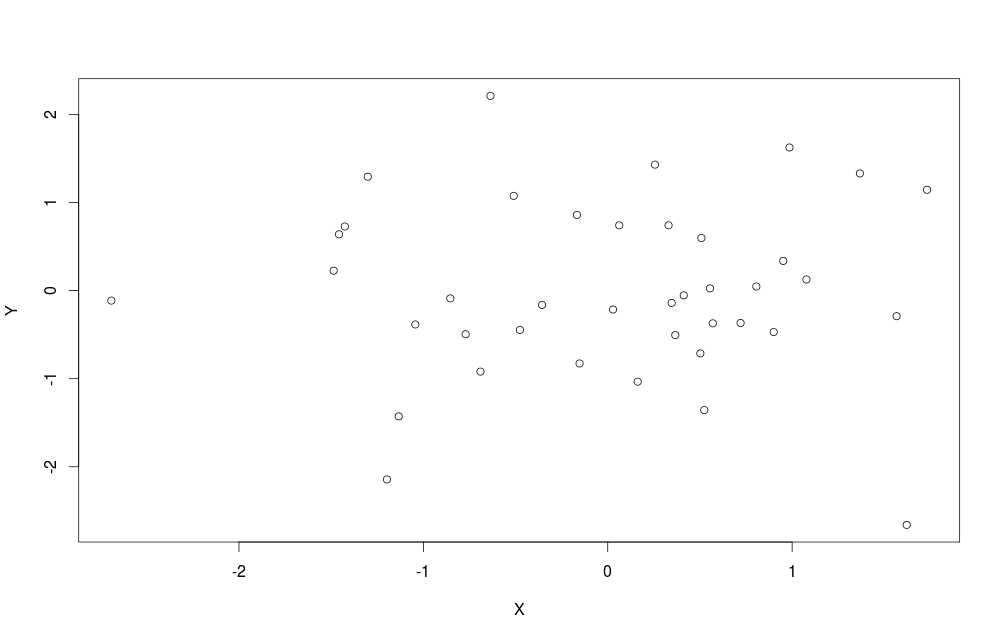
\includegraphics[width=0.9\textwidth]{plot0}
    \caption{Выборка $\rho = 0$}
\end{figure}

\begin{figure}[H]
    \captionsetup{justification=centering}
    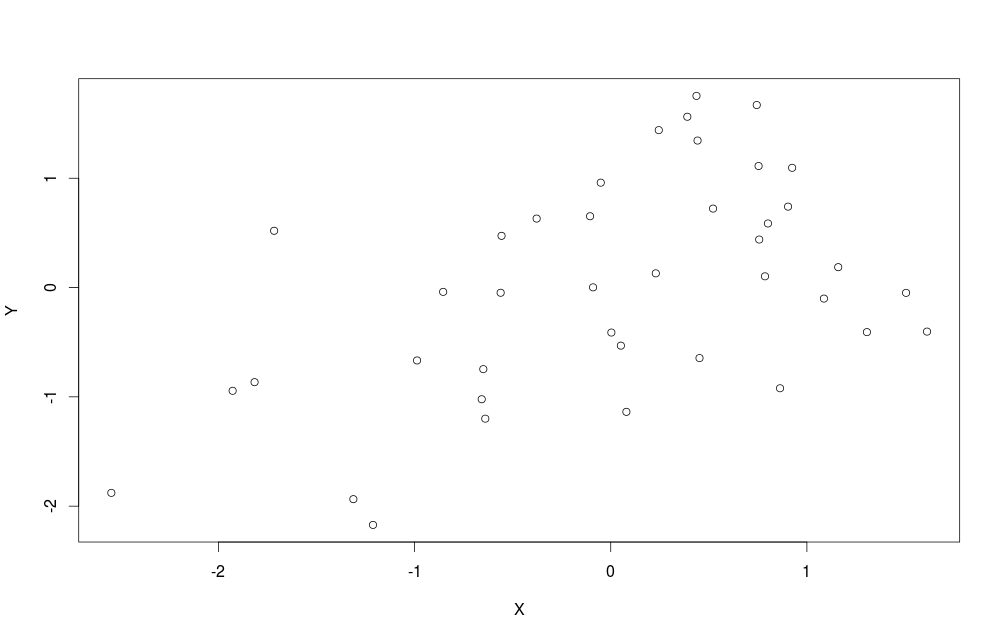
\includegraphics[width=0.9\textwidth]{plot05}
    \caption{Выборка $\rho = 0.5$}
\end{figure}

\begin{figure}[H]
    \captionsetup{justification=centering}
    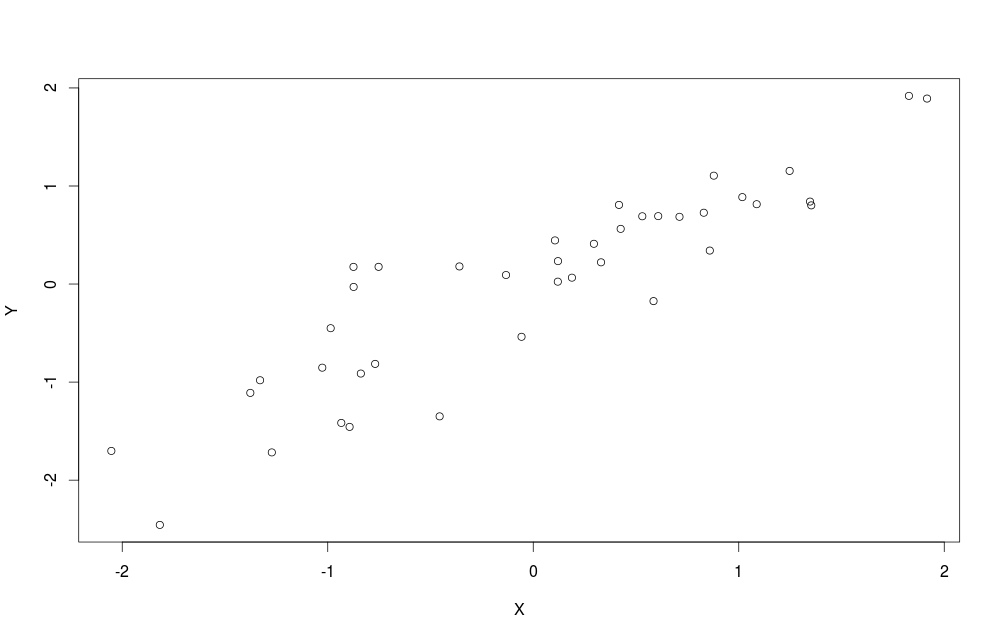
\includegraphics[width=0.9\textwidth]{plot09}
    \caption{Выборка $\rho = 0.9$}
\end{figure}

Ниже представлена таблица с вычисленными характеристиками:
\begin{center}
    \begin{tabular}{|c|c|c|c|c|c|c|c|} 
        \hline
        \rho & r & r_Q & r_S & \tau & r_Q^* & r_S^* & \tau^* \\ 
        \hline
        0 & 0 & 0.1 & 0.038 & 0.038 & 0.156 & 0.040 & 0.060 \\ 
        \hline
        0.5 & 0.5 & 0.4 & 0.428 & 0.285 & 0.588 & 0.444 & 0.432 \\
        \hline
        0.9 & 0.9 & 0.8 & 0.913 & 0.751 & 0.951 & 0.920 & 0.925 \\ 
        \hline
    \end{tabular}
\end{center}

\newpage
Введём в каждую выборку 2 выброса $(-10,10)$ и $(10, -10)$, размер выборок станет соответственно 42:

\begin{figure}[H]
    \captionsetup{justification=centering}
    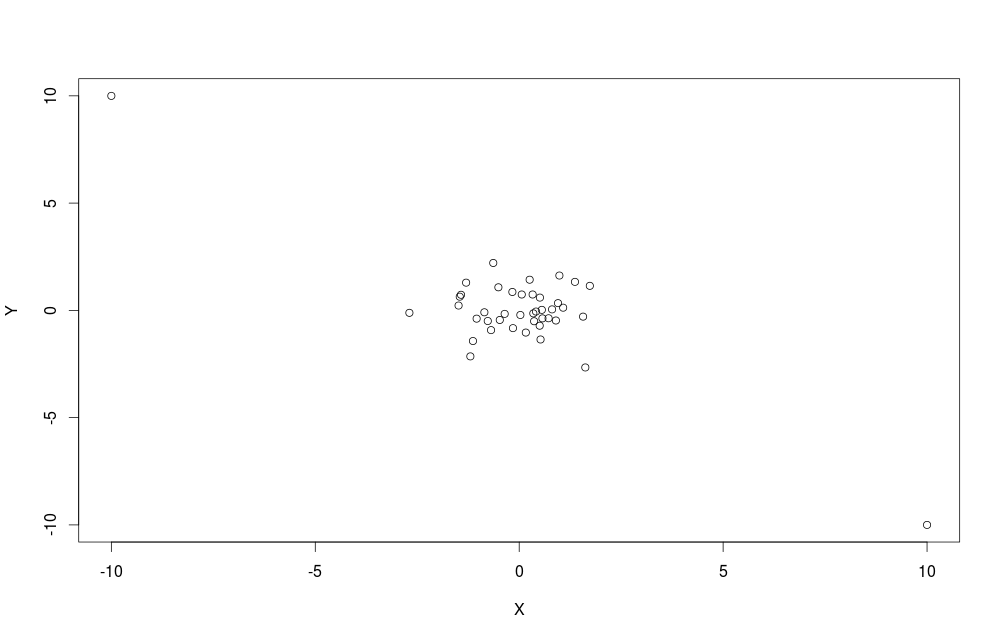
\includegraphics[width=0.9\textwidth]{plot0e}
    \caption{Выборка $\rho = 0$ с выбросами}
\end{figure}

\begin{figure}[H]
    \captionsetup{justification=centering}
    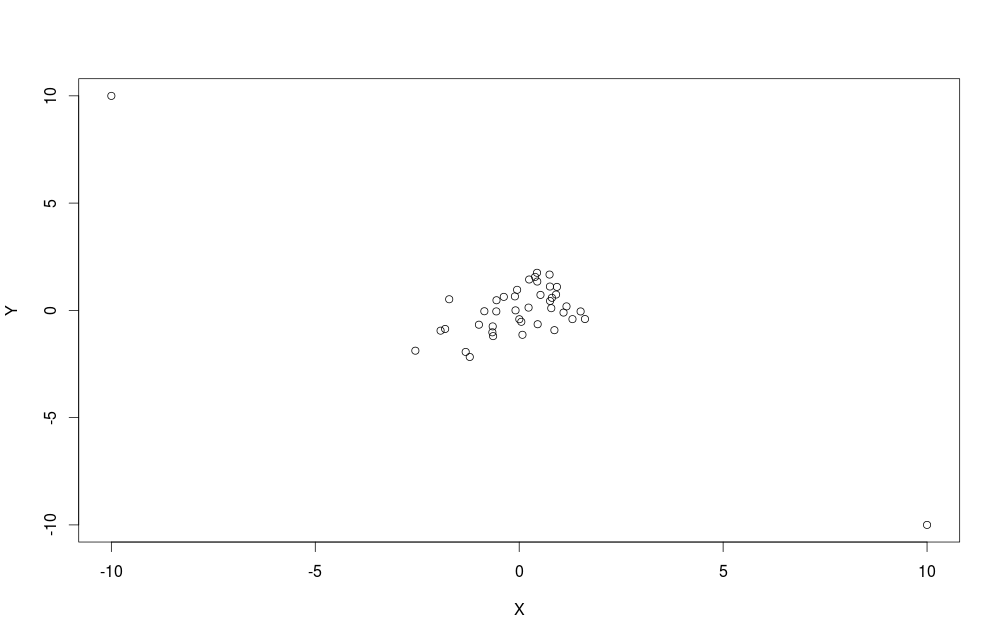
\includegraphics[width=0.9\textwidth]{plot05e}
    \caption{Выборка $\rho = 0.5$ с выбросами}
\end{figure}

\begin{figure}[H]
    \captionsetup{justification=centering}
    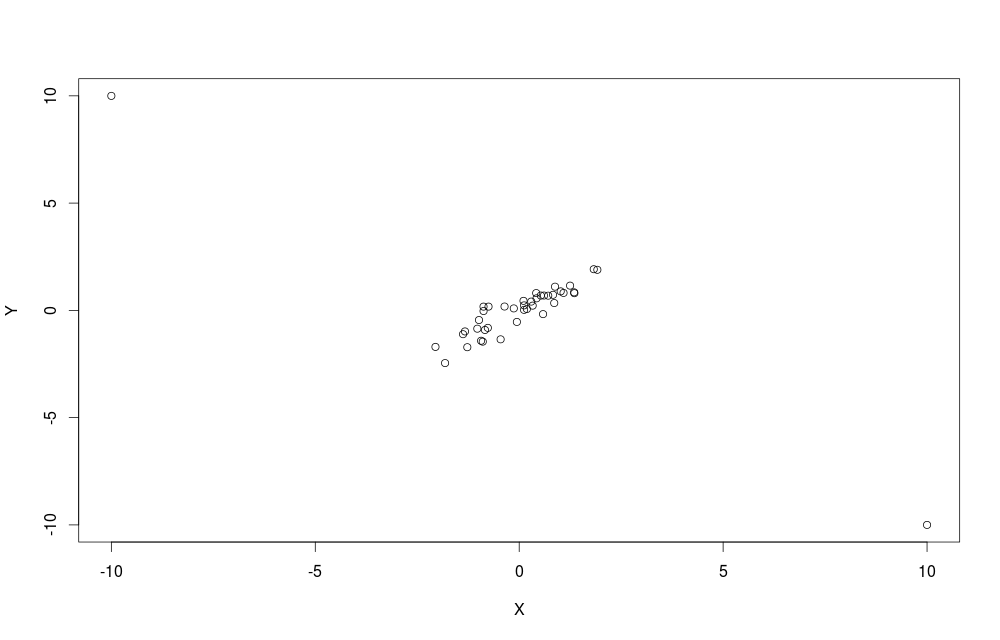
\includegraphics[width=0.9\textwidth]{plot09e}
    \caption{Выборка $\rho = 0.9$ с выбросами}
\end{figure}

Ниже представлена таблица с вычисленными характеристиками для расширенных выборок с выбросами:
\begin{center}
    \begin{tabular}{|c|c|c|c|c|c|c|c|} 
        \hline
        \rho & r & r_Q & r_S & \tau & r_Q^* & r_S^* & \tau^* \\ 
        \hline
        0 & -0.837 & 0.048 & -0.103 & -0.059 & 0.075 & -0.108 & -0.093 \\ 
        \hline
        0.5 & -0.755 & 0.333 & 0.233 & 0.164 & 0.5 & 0.244 & 0.254 \\
        \hline
        0.9 & -0.690 & 0.714 & 0.653 & 0.587 & 0.901 & 0.670 & 0.796 \\ 
        \hline
    \end{tabular}
\end{center}

\section{Заключение}
Из таблиц видно, что в случае без заметных выбросов коэффициент корреляции Пирсона лучше всего совпадает с указанной при генерации данных корреляцией. Остальные коэффициенты тоже дают хороший результат, особенно, когда отнормированны по известным соотношениям.

При добавлении выбросов, почти перпендикулярных линейной регрессии можно заметить, что коэффициент корреляции Пирсона совсем сбивается и больше основывается на этих выбросах, чем на основной выборке. Остальные коэффициенты тоже показывают менее хорошие результаты. Однако знаковый коэффициент корреляции показал результаты даже лучше, чем без выбросов, т.к. основывается на медиане, в отличии от среднего выборочного и на рангах, поэтому влияние единичных заметных выбросов невелируется.

\end{document} % Конец документа
